\documentclass[11pt]{amsart}

% Standard letter size paper with 1inch margins
\usepackage[letterpaper, margin=1in]{geometry}
\usepackage{booktabs} % For better looking tables
\usepackage{xcolor}
\usepackage{pifont}

% Useful packages 
\usepackage{amsmath, amssymb, amsthm, amsaddr}
\usepackage{enumerate, subcaption, graphicx, hyperref}
\usepackage{algorithm}
\usepackage{algpseudocode}
\usepackage{cite}
\usepackage{bm}

\newcommand{\I}{\mathrm{i}}
\DeclareMathOperator{\E}{e}

\title{AMATH 582: Homework 4}
\author{Hunter Lybbert} % first and last name

\address{Applied Mathematics Department, University of Washington, Seattle, WA 
\\ \texttt{hlybbert@uw.edu}}

\date{\today} % you can also just type the date instead of "\today"

\begin{document}

\maketitle

\begin{abstract}
    In this report we survey fully connected linear neural networks and the most common hyperparameters to consider for tuning.
    Various methods of optimization are evaluated with a variety of learning rates and momentums.
    Dropout and batch normalization are discussed and implemented as well.
    Methods of hyperparameter tuning, comparing models and results are presented.
    The task we are applying this to is the well known 10 class classification problem with the FashionMNIST dataset.
\end{abstract}

\section{Introduction and Overview}\label{sec:Introduction}
In this report we further our understanding of machine learning concepts focusing on deep learning, the study of neural network based model architecture.

Again, our setup is a common supervised learning problem, given a collection of $N$ data points with labels in classification or target values in a regression setting $$\big\{(\bm{x_0}, y_0), (\bm{x_1}, y_1), ..., (\bm{x_{N-1}}, y_{N-1})\big\}.$$
The data is denoted as a matrix $X$ and a vector of target values or class labels $\bm y$.
We then are looking for a function $f$ which takes in the training data and most accurately predicts the target values or class labels, written in optimization form we are looking for the following
\begin{equation}
f_{MLE} = \underset{f}{\rm argmin } \frac 1 {2 \sigma^2}|| f(X) - \bm y ||_2^2
\label{eq:basic_ml_setup}
\end{equation}
where $\sigma^2$ is the variance of the normally distributed error terms $\epsilon \sim \mathcal N (0, \sigma^2)$ defined by $\epsilon_i = y_i - f(x_i)$
So said another way we are trying to minimize our errors in the classification task.
The specific class of functions $f$ to be considered to solve the problem is a Fully Connected Neural Network (FCN).
We will treat the theoretical background of these methods in the next section \ref{sec:theory}.

Before proceeding, we would like to acknowledge the critical use of the following packages in our analysis.
Namely, Matplotlib was used to create all plots and animations \cite{Hunter:2007}.
Addiitonally, PyTorch \cite{Ansel_PyTorch_2_Faster_2024} was crucial for easily implementing the desired architecture while Ray Tune \cite{liaw2018tune} was used to help with hyper parameter tuning.

\section{Theoretical Background}\label{sec:theory}
For the purpose of this report we will be concise and straight to the point about the methods, architectures, and hyperparameters used in our study.
The motivation for constructing a neural network is quite literally the network structure of the neurons in our very own brains (see Figure \ref{fig:neuron}).

\begin{figure}[h]
	\centering
	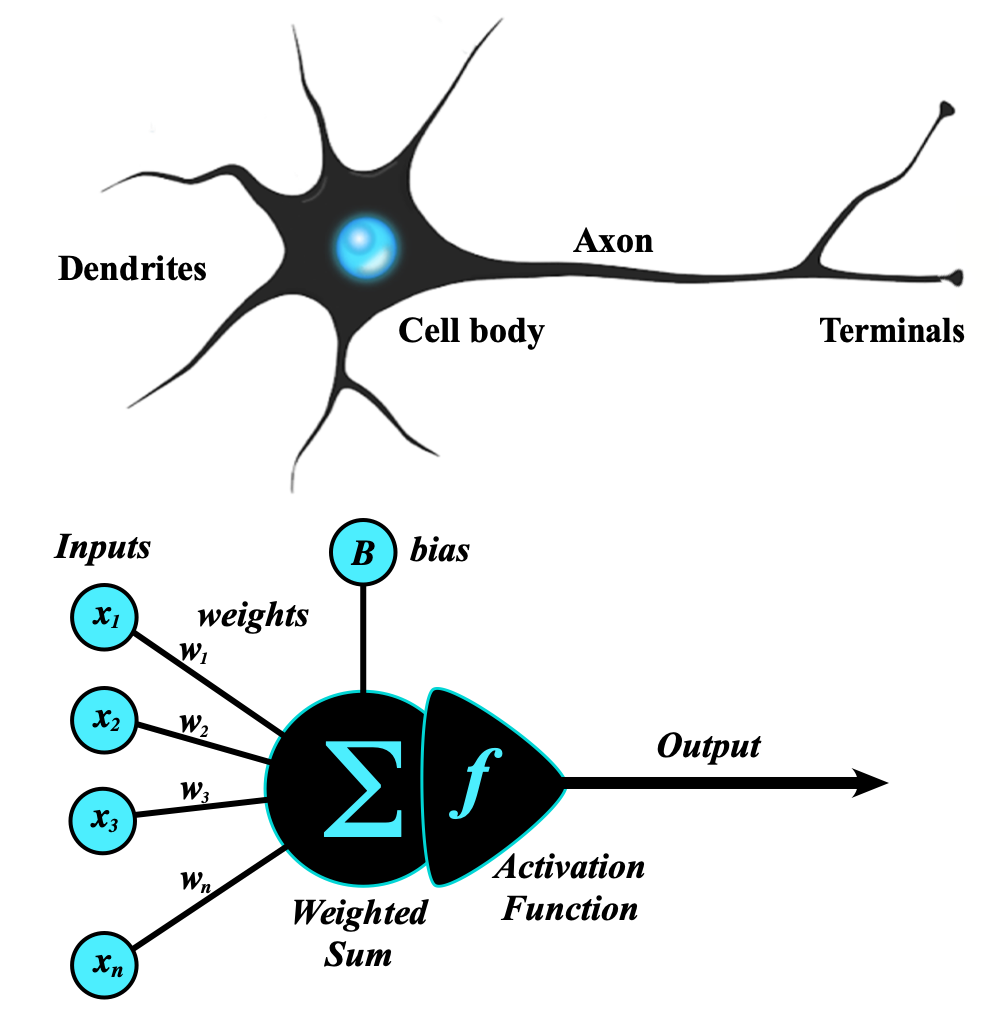
\includegraphics[width=.3\textwidth]{../visualizations/perceptron-with-neuron.png}
 	\caption{Neural networks are truly motivated by the biological behavior of neurons in our brains. (Image from \cite{mriquestionsDeepLearning})}\label{fig:neuron}
\end{figure}

Key components of a biological neuron which are reflected in the artificial neuron in our models are the Dendrites which receive the signals into the neuron, this is like the weights receiving input from the previous layer.
The Cell body combines these signals like our neuron which calculates a weighted sum of the inputs plus a bias (like in regression).
Depending on the signal a neuron received it may fire and pass along the signal through the axon to the neurons down stream from it, artificially our nonlinear activation functions act as this thresholding decision maker determining when to pass on the signal and at what strength to the next layer.
The power of a neural network is creating a large network that is comprised of very wide layers (many neurons) and or is many layers deep.
However, the basic building block is this artificial neuron we have just described.

Another fundamental piece of information to describe, before we get into the architecture and hyperparameters, is what a forward and backward pass through the network are.
Firstly, a forward pass is simply taking the data we are using to try and make predictions of some sort and passing it into the network.
More mathematically we have the following expression for each neuron
\begin{equation}
y = f\left( \sum_{i=1}^n x_i w_i + b \right)
\label{eq:neuron_calc}
\end{equation}
where $x_i$ are the elements of our input vector $\bm x$  or the results of a previous layers output (past $y$'s).
The $w_i$'s are the weights of the connections between these previous layers outputs or original inputs.
We also add a bias term $b$.
Next, the weighted sum is passed through the nonlinear activation function $f$ to produce either a final prediction if this is the final layer in the network or creating the input for the next hidden (not first or last) layer in the network.
Secondly, a backward pass is when we grade how well the network predicted the target output and we propagate the information about how wrong we were back through the network to improve our prediction a little for the next forward pass.
Once again, we have a more concise mathematical expression for this, which we will get to momentarily.
Recall the expression \eqref{eq:basic_ml_setup} which we are trying to argmin, this metric or measure of error we are trying to minimize is called a loss function.
We can choose different loss functions, let's denote our arbitrary choice of loss function as $L(\hat y, y)$ where $\hat y$ is the predicted label or value from the network and $y$ is the target value or label.
Now we can precisely define backward pass
\begin{equation}
\nabla_{\bm w} L(\hat y, y) = \frac {\partial L}{\partial \hat y} \frac {\partial \hat y}{\partial z} \nabla_{\bm w} z.
\label{eq:back_prop}
\end{equation}
We are referring to variables as represented here in this more graphical representation of forward and backward passes
\begin{align*}
\boxed{\bm w^T \bm x + b = z} \rightarrow \boxed{\sigma(z) = \hat y} \rightarrow \boxed{L(\hat y , y)} \\
\boxed{\nabla_{\bm w} z} \leftarrow \boxed{\frac {\partial \hat y}{\partial z} (z)} \leftarrow \boxed{\frac {\partial L}{\partial \hat y}(\hat y , y)}.
\end{align*}
For completion and yet in favor of being concise, we include the following expression for gradient descent which is how we update the weights is
\begin{align*}
\bm w_{k + 1} &= \bm w_{k} - \alpha \nabla_{\bm w} J(\bm w_{k}; b) \\
b_{k + 1} &= b_{k} - \alpha \frac \partial {\partial b}J(\bm w; b_k).
\label{eq:gd}
\end{align*}
There is, of course, more to say about exactly how back propogation works or how autograd works in pytorch but for the sake of this report we will leave it here and begin our discussion of the optimizers and hyperparameters.

\subsection{Architecture}
The first decision one needs to make when considering a neural network to solve the problem at hand

\subsection{Optimizer}
\textbf{TODO: Update}
Talk about, learning rates, and momentum
\begin{enumerate}
\item SGD
\item Adam
\item RMSProp
\end{enumerate}

\subsection{Dropout}
\textbf{TODO: Update}
Describe briefly why we do this to avoid overfitting

\subsection{Batch Normalization}
\textbf{TODO: Update}
Describe how this helps things be a little more stable

\subsection{Weight Initialization}
\textbf{TODO: Update}
Describe how the starting point matters a lot on such a complicated loss surface

\section{Algorithm Implementation and Development}\label{sec:algorithms}
\textbf{TODO: Update}
\begin{enumerate}
\item discuss how you implemented the model architecture with variable layers and sizes
\item discuss how you tried to implement Ray Tune
\item Describe your ModelTrainingArtifact Class
\item Describe how you chose to hyperparameter tune across all hps instead of doing it incrementally (for the sake of thoroughness).
\item Describe how you logged the experiment results and the short comings of that.
\end{enumerate}

\section{Computational Results}\label{sec:results}

\textbf{TODO: Update}


\begin{figure}[h]
	\centering
	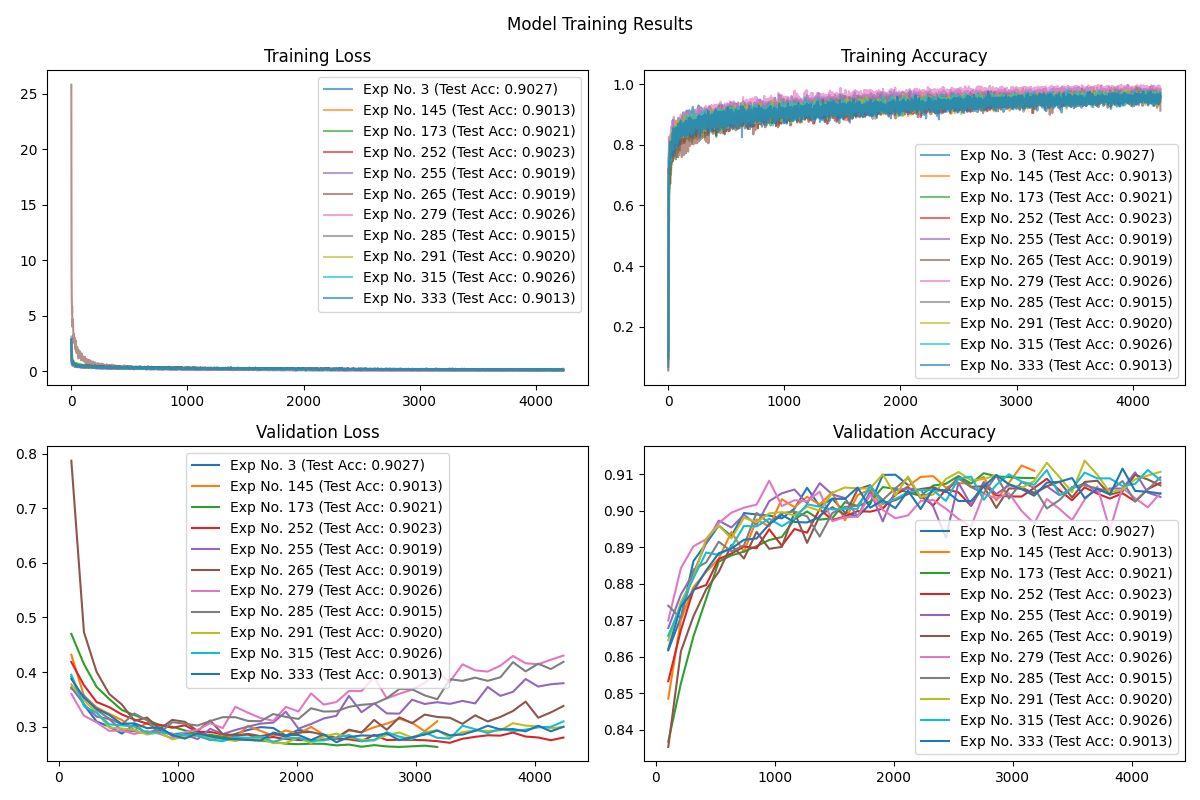
\includegraphics[width=.9\textwidth]{../visualizations/model_training_results_vis.png}
 	\caption{\textbf{TODO: Update caption}}\label{fig:f0}
\end{figure}

\begin{figure}[h]
	\centering
	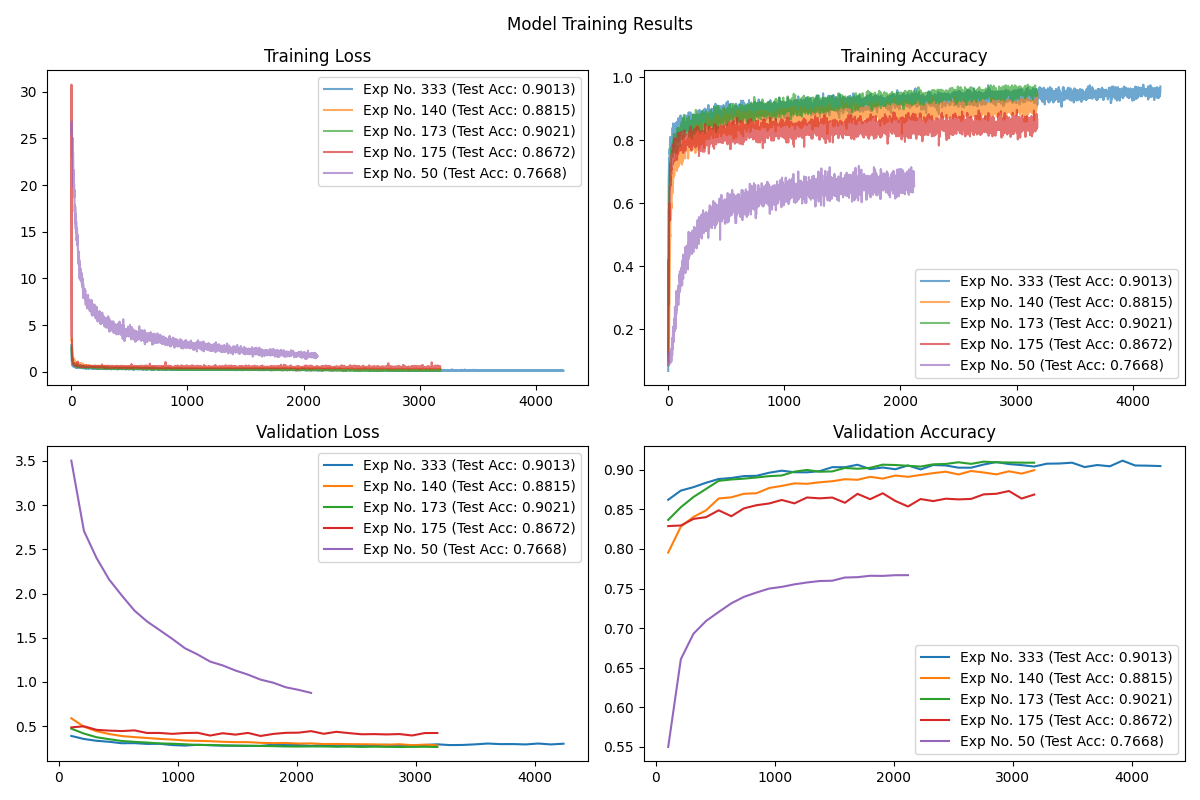
\includegraphics[width=.9\textwidth]{../visualizations/model_training_results_vis_0.png}
 	\caption{\textbf{TODO: Update caption}}\label{fig:f1}
\end{figure}

\begin{figure}[h]
	\centering
	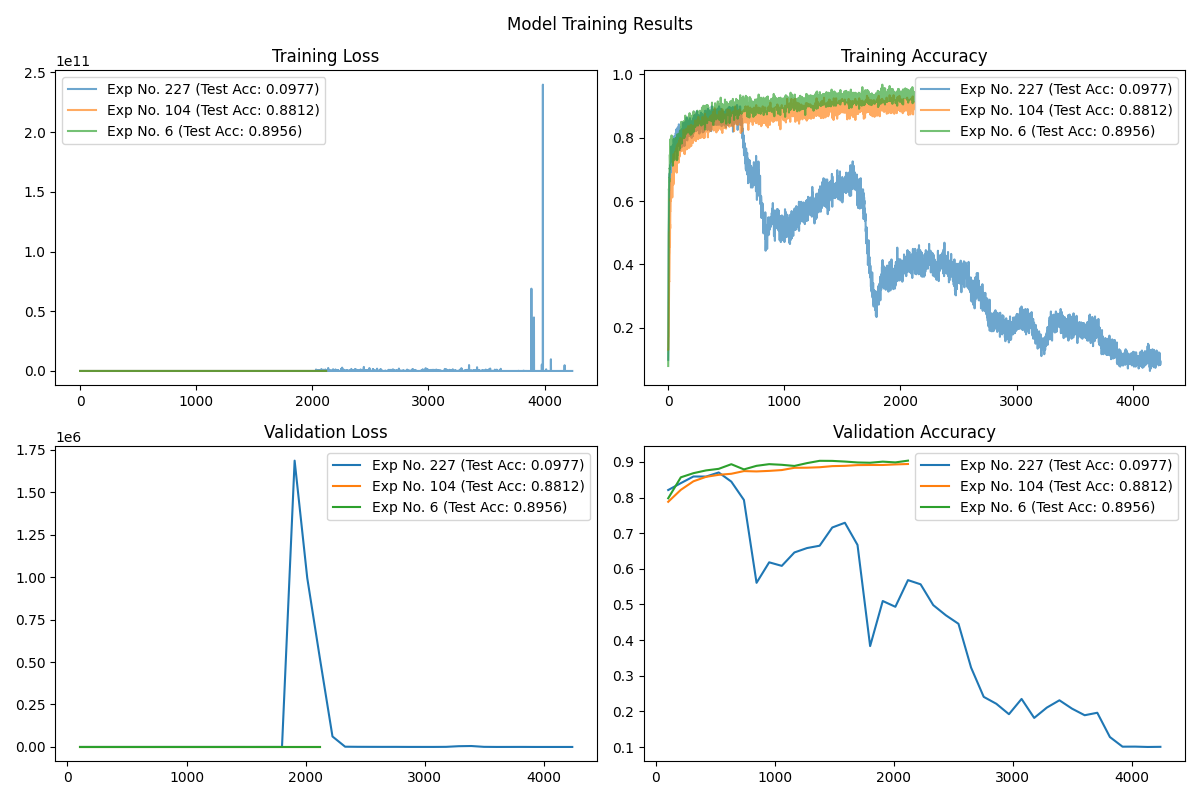
\includegraphics[width=.9\textwidth]{../visualizations/model_training_results_vis_1.png}
 	\caption{\textbf{TODO: Update caption}}\label{fig:f2}
\end{figure}

\begin{figure}[h]
	\centering
	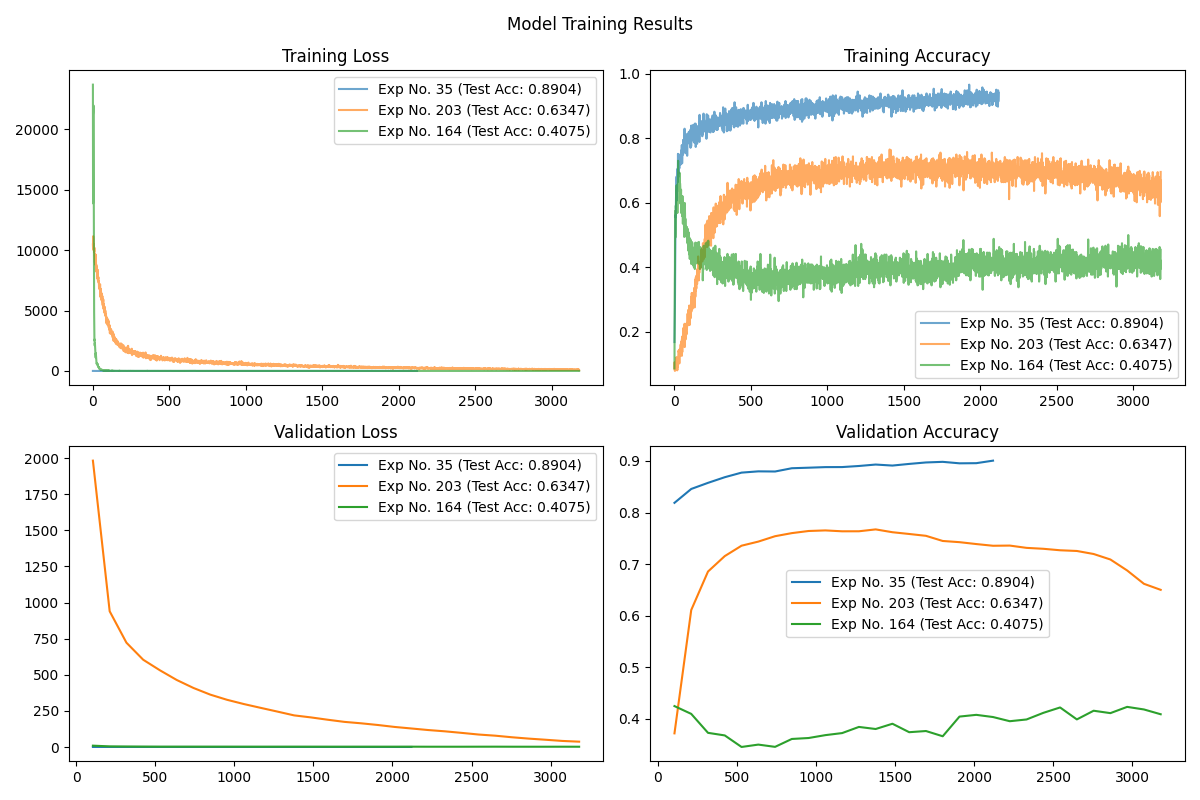
\includegraphics[width=.9\textwidth]{../visualizations/model_training_results_vis_2.png}
 	\caption{\textbf{TODO: Update caption}}\label{fig:f3}
\end{figure}

\begin{table}[h]
    \centering
    \begin{tabular}{|l|c|c|c|c|} % 'l' for left-aligned, 'c' for center-aligned columns
        \hline
        \textbf{Classifier} & \textbf{Digits Used} & \textbf{Train Accuracy} & \textbf{Test Accuracy} & \textbf{CV Score} \\ 
        \hline
        Ridge Classifier & 1 and 8 & 0.965  & 0.980 & 0.963 $\pm$ 0.00281 \\
        \hline
        Ridge Classifier & 3 and 8 & 0.961  & 0.964 & 0.959 $\pm$ 0.00590 \\
        \hline
        Ridge Classifier & 2 and 7 & 0.981  & 0.973 & 0.981 $\pm$ 0.00226 \\  
        \hline
    \end{tabular}
    \caption{\textbf{TODO: update me}}
    \label{tab:tab0}
\end{table}


\section{Summary and Conclusions}\label{sec:conclusions} 
\textbf{TODO: Update}
\begin{enumerate}
\item further work is going to include finding a better way to share and convey the configuration in the visuals
\item screw ray tune
\end{enumerate}

\section*{Acknowledgements}
\textbf{TODO: Update}
The author is thankful to Jaxon Tuggle, Hailey Sparks, Anja Vogt, Jade Glaister, and Nate Ward for offering regular feedback and counsel when interpreting results and clarifying the implications and merits of different classifiers.
We would also like to thank Professor Eli Shlizerman for carefully instructing us in class.

\bibliographystyle{abbrv}
\bibliography{references_hw4} % make sure this matches the .bib file for your corresponding document. You also have to maintain your references in the .bib file 

\end{document}
